\phantomsection
\chapter{Results}
\label{chap:eval_results}

\noindent Two kinds of results have been obtained. The first results are obtained by using a test set from the database used for the training set. The LBP operator extract features from each image of the test set, then the classification is done and this is how the first result set is obtained. The second result set is obtained with the Kinect. The Kinect gets video sequences of a subject in front of the Kinect and from these sequences, face images are extracted. Then the same process is applied to these face images and that is where comes from the second result set.
\newline

\phantomsection
\section{First result set}

\vspace{\baselineskip}
\noindent To train the model, 128 face images from the KDEF database have been used for each emotion plus the neutral state. In total, $ 128\times7 = 896 $ face images have been used to train the model. To test the model, 12 face images from the KDEF database have been used for each emotion plus the neutral state. In total, $ 12\times7 = 84 $ faces images has been used to test the model. For each of these 84 images, face detection was used first, then the LBP operator to extract the features and then the classification method was used.
\newline

\noindent For the classification part, the data has been trained with different kernels and different parameters. The following table resumes the results that have been obtained:
\newline

\vspace{\baselineskip}
\begin {center}
\begin{tabular}{|c|c|c|c|c|c|c|c|c|}
  \hline
    & Linear & Poly1 & Poly2 & RBF1 & RBF2 & Sigmoid1 & Sigmoid2 \\
  \hline
  neutral & 33.33\% & 33.33\% & 25.00\% & 33.33\% & 33.33\% & 58,33\% & 41.67\% \\
  afraid & 66.67\% & 91.67\% & 100.00\% & 75.00\% & 83.33\% & 75.00\% & 75.00\% \\
  angry & 50.00\% & 50.00\% & 41.67\% & 50.00\% & 50.00\% & 66.67\% & 50.00\% \\
  disgusted & 75.00\% & 83.33\% & 83.33\% & 75.00\% & 75.00\% & 75.00\% & 83.33\% \\
  happy & 91.67\% & 91.67\% & 91.67\% & 91.67\% & 91.67\% & 91.67\% & 91.67\% \\
  sad & 16.67\% & 16.67\% & 8.33\% & 8.33\% & 8.33\% & 8.33\% & 16.67\% \\
  surprised & 33.33\% & 58.33\% & 50.00\% & 66.67\% & 58.33\% & 50.00\% & 75.00\% \\
  overall & 52.38\% & 60.71\% & 57.14\% & 57.14\% & 57.14\% & 60.71\% & 61.90\% \\
  \hline
\end{tabular}
\end {center}

\vspace{\baselineskip}
\vspace{\baselineskip}
\noindent Poly1 stands for Polynomial and has this parameter: $ D = 2 $
\newline
\noindent Poly2 stands for Polynomial and has this parameter: $ D = 3 $
\newline
\noindent RBF1 has these parameters: $ C = 8.0 $ and $ \gamma = 0.0078125 $
\newline
\noindent RBF2 has these parameters: $ C = 32.0 $ and $ \gamma = 0.001953125 $ 
\newline
\noindent Sigmoid1 has these parameters: $ C = 8.0 $ and $ \gamma = 0.0078125 $
\newline
\noindent Sigmoid2 has these parameters: $ C = 32.0 $ and $ \gamma = 0.001953125 $
\newline

\noindent The same data has been trained with the same kernels and parameters but using the cross validation method (as explained in \ref{chap:implementation_svm}). All the results, compared to the one obtained without using cross validation are worse. Following is a table of both results with and without cross validation.
\newline

\vspace{\baselineskip}
\begin {center}
\begin{tabular}{|c|c|c|c|c|c|c|c|c|}
  \hline
    & with cross validation & without cross validation \\
  \hline
  Linear & 53.57\% & 52.38\% \\
  Poly1 & 54.76\% & 60.71\% \\
  Poly2 & 44.05\% & 57.14\% \\
  RBF1 & 55.95\% & 57.14\% \\
  RBF2 & 50.00\% & 57.14\% \\
  Sigmoid1 & 55.95\% & 60.71\% \\
  Sigmoid2 & 61.90\% & 61.90\% \\
  \hline
\end{tabular}
\end {center}

\vspace{\baselineskip}
\vspace{\baselineskip}
\noindent The best accuracy percentage is for the Sigmoid2 column. It is obtained with a classification based on the Sigmoid kernel and with the following parameters for this kernel: $ C = 32.0 $ and $ \gamma = 0.001953125 $. These parameters are found by \textit{gridsearch}, a script of the SVM library. They are the most optimized for the RBF kernel and for the Sigmoid kernel. The overall percentage of accuracy for all the emotions is $ 61.90\% $. Following is the confusion matrix:
\newline

\vspace{\baselineskip}
\begin {center}
\begin{tabular}{|c|c|c|c|c|c|c|c|c|}
  \hline
   & neutral & afraid & angry & disgusted & happy & sad & surprised & accuracy \\
  \hline
  neutral & 5 & 4 & 2 & 0 & 1 & 0 & 0 & 41.67\% \\
  afraid & 0 & 9 & 0 & 0 & 0 & 2 & 1 & 75.00\% \\
  angry & 2 & 3 & 6 & 0 & 0 & 1 & 0 & 50.00\% \\
  disgusted & 0 & 1 & 0 & 10 & 0 & 1 & 0 & 83.33\% \\
  happy & 0 & 0 & 0 & 1 & 11 & 0 & 0 & 91.67\% \\
  sad & 0 & 4 & 3 & 1 & 2 & 2 & 0 & 16.67\% \\
  surprised & 2 & 1 & 0 & 0 & 0 & 0 & 9 & 75.00\%\\
  \hline
\end{tabular}
\end {center}

\vspace{\baselineskip}
\vspace{\baselineskip}
\noindent By looking at the confusion matrix, it is easy to notice that 3 facial expressions are harder to recognize than the others with this system. These 3 emotions are: angry, sad and neutral. There is a real gap between these 3 emotions and the 4 other ones (afraid, disgusted, happy and surprised). Indeed, these 3 emotions are recognized with an accuracy lower than $ 50\% $, while the 4 other ones are recognized with an accuracy higher than $ 70\% $.
\newline

\vspace{\baselineskip}
\begin {center}
\begin{tabular}{|c|c|c|c|c|c|c|c|c|}
  \hline
   $ < 50\% $ & > 75\% \\
  \hline
  neutral ($ 5/12 $) & afraid ($ 9/12 $) \\
  angry ($ 6/12 $) & disgusted ($ 10/12 $) \\
  sad ($ 2/12 $) & happy ($ 11/12 $) \\
   & surprised ($ 9/12 $) \\
  \hline
\end{tabular}
\end {center}

\vspace{\baselineskip}
\vspace{\baselineskip}
\noindent The numbers that are in parenthesis represent the number of emotions well recognized over the total number of face images tested.
\newline

\noindent These 6 emotions plus the neutral state can be classified into 2 groups. Indeed, one group containing the 3 emotions hard to recognize and the second group containing the 4 emotions remaining. The 3 facial expressions \textit{angry}, \textit{sad} and \textit{neutral}, are the ones that distort the less the face. Between 3 faces expressing each,  one of these emotions, the differences are not clearly noticeable. The figure~\ref{kdef_no_difference_emotions} shows face images from the KDEF database used in the test set, expressing these 3 facial expressions.
\newline

\begin{figure}[!h]
\begin{center}
\noindent 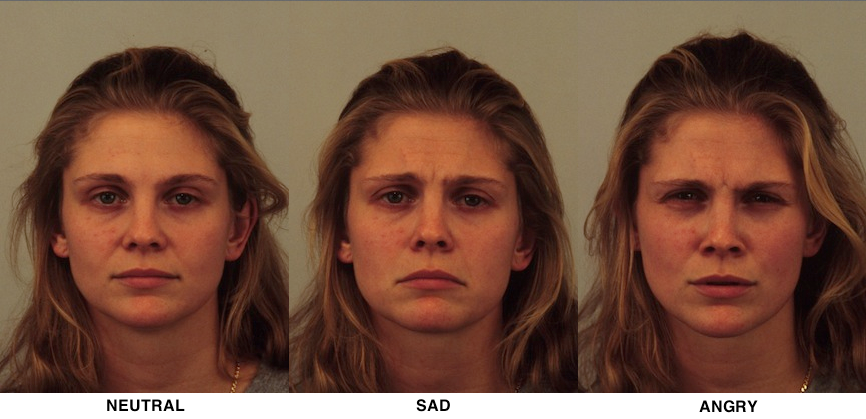
\includegraphics[scale=0.4]{figures/kdef_no_difference_emotions} 
\newline
\caption{Face images from the KDEF database used in the test set}
\label{kdef_no_difference_emotions}
\end{center} 
\end{figure}

\noindent The second group contains the 4 following facial expressions \textit{afraid}, \textit{disgusted}, \textit{happy} and \textit{surprised}. These emotions distort significantly the face when they are expressed. This is why it is easier to recognize them. The figure~\ref{kdef_difference_emotions} shows face images from the KDEF database used in the test set, expressing these 4 facial expressions. The important features carrying emotion as the mouth or the eyes are changing a lot while these 4 emotions are expressed.
\newline

\begin{figure}[!h]
\begin{center}
\noindent 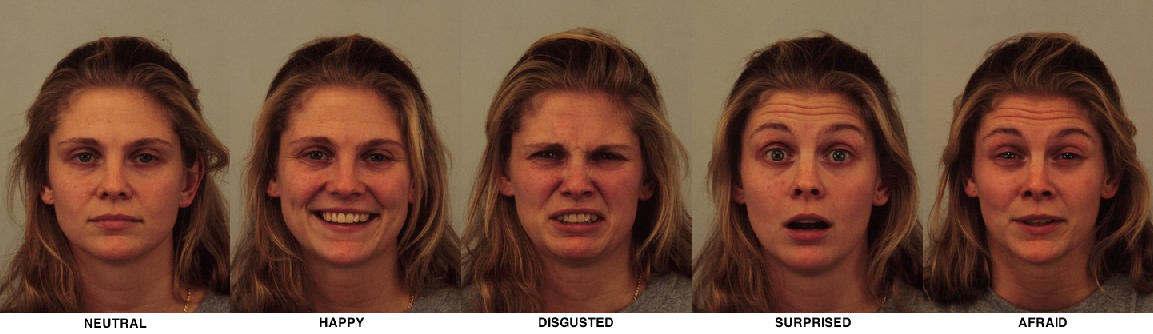
\includegraphics[scale=0.3]{figures/kdef_difference_emotions} 
\newline
\caption{Face images from the KDEF database used in the test set}
\label{kdef_difference_emotions}
\end{center} 
\end{figure}

\noindent As can be seen in the figure~\ref{kdef_difference_emotions}, for each emotion, the eyebrows are raised, or the eyes are wild opened and most of the the mouth is clearly opened. For the figure~\ref{kdef_no_difference_emotions}, nothing is clearly noticeable, the face is almost the same. All of this can explain the difficulties that the system encounters to differentiate the emotions \textit{angry}, \textit{sad} and \textit{neutral}.
\newline

\phantomsection
\section{Second result set}

\vspace{\baselineskip}
\noindent The second result test is obtained based on the same process than the process that gives the first result set. The only difference is the input. The input is not face image from which the features are extracted; it is a video stream from the Kinect. A subject stands in face of the Kinect, the face is detected, then the features are extracted, and finally the classification is made almost in real time and the output is the name of the emotion expressed.
\newline

\noindent GIVE THE RESULTS OBTAINED
\newline

